% Opsætter KU Tex dokument
%%%%%%%%%%%%%%%%%%%%%%%%%%%%%%%%%%%%%%%%%%%%%%%%%%%%%%%%%%%%%%%%%%%%%%%%%%%%%%%%
\documentclass{article}                                                        %
\usepackage[a4paper, hmargin={2.8cm, 2.8cm}, vmargin={2.5cm, 2.5cm}]{geometry} %
\usepackage{eso-pic}  % \AddToShipoutPicture                                   %
\usepackage{graphicx} % \includegraphics                                       %
\usepackage{setspace}                                                        %
%%%%%%%%%%%%%%%%%%%%%%%%%%%%%%%%%%%%%%%%%%%%%%%%%%%%%%%%%%%%%%%%%%%%%%%%%%%%%%%%

% Pakker til skrifttyper, tekst osv.
%%%%%%%%%%%%%%%%%%%%%%%%%%%%%%%%%%%%%%%%%%%%%%%%%%%%%%%%%%%%%%%%%%%%%%%%%%%%%%%%
    \usepackage[utf8]{inputenc}  % Implementere Unicode                        %
    \usepackage[T1]{fontenc}     % Unicode skrifttype fx. é skrives som 1 tegn %
    \usepackage[english]{babel}   % Dansk Ordbog                                %
    \usepackage{microtype}       % Forbedre linjeombrydningen                  %
    \usepackage{libertine}       % Skrifttype                                  %
%%%%%%%%%%%%%%%%%%%%%%%%%%%%%%%%%%%%%%%%%%%%%%%%%%%%%%%%%%%%%%%%%%%%%%%%%%%%%%%%

% Pakker til matematik og kode.
%%%%%%%%%%%%%%%%%%%%%%%%%%%%%%%%%%%%%%%%%%%%%%%%%%%%%%%%%%%%%%%%%%%%%%%%%%%%%%%%
    \usepackage{mathtools}       % Udvidelse til amsmath pakken                %
    \usepackage{amsthm}          % Pakke til bevisførelse                      %
    \usepackage{amssymb}         % Extra matematiske symboler                  %				
	\usepackage{mychemistry}												   %
	\usepackage[version=3]{mhchem}											   %
	\usepackage{wrapfig}													   %
	\usepackage{siunitx}	
	\usepackage{anyfontsize}
	\usepackage{ragged2e}
	\usepackage{algorithm2e}
	\usepackage[final]{pdfpages}
	\usepackage{listings}
	\usepackage{tikz}
	\usepackage{multirow}
	\usepackage{makecell}
	\usepackage{fourier} 
	\usepackage{array}
	\usepackage{todonotes}
	\usepackage{pdflscape}
	\usetikzlibrary{arrows,shapes}
	\usepackage{titlesec}
	\usepackage{hyperref}
	\usepackage{url}
	\usepackage[nottoc,numbib]{tocbibind}
	\usepackage{subcaption} %\usepackage{subfig}    
	
	\urlstyle{same}
	\tikzstyle{vertex}=[circle,fill=white!25,minimum size=20pt,inner sep=0pt]
	\tikzstyle{edge} = [draw,thick,-]

	\definecolor{light-gray}{gray}{0.85}
	\definecolor{dkgreen}{RGB}{0.0,128.0,43.0}
	\lstdefinelanguage{FSharp}%
{morekeywords={new, match, with, rec, open, module, namespace, type, of, member, % 
and, for, while, true, false, in, do, begin, fun, function, return, yield, try, %end
mutable, if, then, else, cloud, async, static, use, abstract, interface, inherit, finally, int },
  otherkeywords={ let!, return!, do!, yield!, use!, var, from, select, where, order, by },
  keywordstyle=\color{bluekeywords},
  sensitive=true,
  basicstyle=\ttfamily,
	breaklines=true,
  xleftmargin=\parindent,
  aboveskip=\bigskipamount,
	tabsize=4,
  morecomment=[l][\color{dkgreen}]{///},
  morecomment=[l][\color{dkgreen}]{//},
  morecomment=[l][\color{dkgreen}]{(*},
  morecomment=[s][\color{dkgreen}]{},
  morestring=[b]",
  showstringspaces=false,
  literate={`}{\`}1,
  stringstyle=\color{redstrings},
}
	
	\lstset{frame=tb,
  	language=FSharp,			%CHANGE LANGUAGE
  	aboveskip=3mm,
  	belowskip=3mm,
  	showstringspaces=false,
  	columns=flexible,
  	basicstyle={\small\ttfamily},
  	numbers=none,
  	numberstyle=\tiny\color{gray},
  	keywordstyle=\color{blue},
  	commentstyle=\color{dkgreen},
  	stringstyle=\color{red},
  	breaklines=true,
  	breakatwhitespace=true,
  	tabsize=3,
  	backgroundcolor=\color{light-gray},
	}
												   %
%%%%%%%%%%%%%%%%%%%%%%%%%%%%%%%%%%%%%%%%%%%%%%%%%%%%%%%%%%%%%%%%%%%%%%%%%%%%%%%%

% Pakker til layout.
%%%%%%%%%%%%%%%%%%%%%%%%%%%%%%%%%%%%%%%%%%%%%%%%%%%%%%%%%%%%%%%%%%%%%%%%%%%%%%%%
    \usepackage{fancyhdr}            % Gør det muligt at bruge sidehoveder     %
    \usepackage{graphicx}            % Mulighed for bl.a. \includegraphics     %
    \usepackage{colortbl}            % Hvis man vil farvelægge sine tabeller   %
    \usepackage{array}               % Gør miljøerne array og tabular bedre    %
    \usepackage{parskip}             % Første paragraf i afsnit indrykkes ikke %
    \usepackage{titlesec}            % Tilpassing af afstand mellem sektioner  %
    \usepackage[lastpage,user]{zref} % Side x af y                             %
%%%%%%%%%%%%%%%%%%%%%%%%%%%%%%%%%%%%%%%%%%%%%%%%%%%%%%%%%%%%%%%%%%%%%%%%%%%%%%%%


% Implementerer en række makroer og de pakker der er importeret
%%%%%%%%%%%%%%%%%%%%%%%%%%%%%%%%%%%%%%%%%%%%%%%%%%%%%%%%%%%%%%%%%%%%%%%%%%%%%%%%
    \pagestyle{fancy}                        % Implementerer sidehoved         %
    \lhead{University of Copenhagen}                % Venstre sidehoved               %
    \rhead{Casper Bresdahl}                             % Højre sidehoved      %
    \cfoot{\thepage\ of \zpageref{LastPage}} % Side x af y                     %
    \newtheorem*{prp}{Propostion}            % Skaber nyt theorem  
    \renewcommand{\baselinestretch}{1.5}       %
%%%%%%%%%%%%%%%%%%%%%%%%%%%%%%%%%%%%%%%%%%%%%%%%%%%%%%%%%%%%%%%%%%%%%%%%%%%%%%%%

% Mindsker afstanden mellem sektioner
%%%%%%%%%%%%%%%%%%%%%%%%%%%%%%%%%%%%%%%%%%%%%%%%%%%%%%%%%%%%%%%%%%%%%%%%%%%%%%%%%%
\titlespacing\section{0pt}{12pt plus 4pt minus 2pt}{0pt plus 1pt minus 3pt}      %
\titlespacing\subsection{0pt}{12pt plus 4pt minus 2pt}{0pt plus 1pt minus 3pt}   %
\titlespacing\subsubsection{0pt}{12pt plus 4pt minus 2pt}{0pt plus 1pt minus 3pt}%
%%%%%%%%%%%%%%%%%%%%%%%%%%%%%%%%%%%%%%%%%%%%%%%%%%%%%%%%%%%%%%%%%%%%%%%%%%%%%%%%%%

%Ændrer størelsen på sections
%%%%%%%%%%%%%%%%%%%%%%%%%%%%%%%%%%%%%%%%%%%%%%%%%%%%%%%%%%%%%%%%%%%%%%%%%%%%%%%%%%
\titleformat{\section}
{\normalfont\fontsize{14}{16}\bfseries}{\thesection}{1em}{}
\titleformat{\subsection}
{\normalfont\fontsize{12}{14}\bfseries}{\thesubsection}{1em}{}
\titleformat{\subsubsection}
{\normalfont\fontsize{11}{13}\bfseries}{\thesubsubsection}{1em}{}
%%%%%%%%%%%%%%%%%%%%%%%%%%%%%%%%%%%%%%%%%%%%%%%%%%%%%%%%%%%%%%%%%%%%%%%%%%%%%%%%%%

%%%%%%%%%%%%
% Document %
%%%%%%%%%%%%

\begin{document}

\begin{titlepage}

\newcommand{\HRule}{\rule{\linewidth}{0.5mm}} % Defines a new command for the horizontal lines, change thickness here

\begin{center}
 % Center everything on the page
 
%----------------------------------------------------------------------------------------
%	HEADING SECTIONS
%----------------------------------------------------------------------------------------

\textsc{\LARGE University of Copenhagen}\\[1.5cm] % Name of your university/college
\textsc{\Large Computer Science}\\[0.5cm] % Major heading such as course name
\textsc{\large Image and Vision Processing}\\[0.5cm] % Minor heading such as course title

%----------------------------------------------------------------------------------------
%	TITLE SECTION
%----------------------------------------------------------------------------------------

\HRule \\[0.4cm]
{ \huge \bfseries Assignment 1}\\[0.4cm] % Title of your document
\HRule \\[1.5cm]
 
%----------------------------------------------------------------------------------------
%	AUTHOR SECTION
%----------------------------------------------------------------------------------------

\begin{minipage}{0.4\textwidth}
\begin{flushleft} \large
\emph{Author:}\\ 
% Your name
Casper \textsc{Bresdahl} \\
\end{flushleft}
\end{minipage}
~
\begin{minipage}{0.4\textwidth}
\begin{flushright} \large
\emph{Teacher:} \\
Francois \textsc{Lauze}\\
\end{flushright}
\end{minipage}\\[2cm]

% If you don't want a supervisor, uncomment the two lines below and remove the section above
%\Large \emph{Forfattere:}\\
%Axel \textsc{Christof}\\% Your name
%Casper \textsc{Bresdahl}\\
%Emilie \textsc{Bentsen}\\[1cm] 

%----------------------------------------------------------------------------------------
%	DATE SECTION
%----------------------------------------------------------------------------------------

{\large \today}\\[2cm] % Date, change the \today to a set date if you want to be precise

%----------------------------------------------------------------------------------------
%	LOGO SECTION
%----------------------------------------------------------------------------------------


\includegraphics{logo.png}\\[1cm] % Include a department/university logo - this will require the graphicx package
 
%----------------------------------------------------------------------------------------

\vfill % Fill the rest of the page with whitespace

%Disse linjer skaber forside, evt indholdsfortegnelse, og sætter sidetal
%%%%%%%%%%%%%%%%%%%%%%%%%%%%%%%%%%%%%%%%%%%%%%%%%%%%%%%%%%%%%%%%%%%%%%%%%%%%%%%%
									                                           %
    \thispagestyle{empty}   % Fjerner sidetal forside                          %
        % Slå disse til hvis der ønskes indholdsfortegnelse                    %
        %%%%%%%%%%%%%%%%%%%%%%%%%%%%%%%%%%%%%%%%%%%%%%%%%%%%%%%%%%%%%%%%%%%%%%%% 
            \newpage                % Side til indholdsfortegnelse            %
            \thispagestyle{empty}   % Fjerner sidetal fra indholdsfortegnelse %
            \tableofcontents        % Skaber indholdsfortegnelse              %
    \end{center}
    %\section*{Forord}
    	
		
        %%%%%%%%%%%%%%%%%%%%%%%%%%%%%%%%%%%%%%%%%%%%%%%%%%%%%%%%%%%%%%%%%%%%%%%%
    \newpage                % Første rigtige side
    \setcounter{page}{1}    % Sætter rigtigt sidetal på første side
%%%%%%%%%%%%%%%%%%%%%%%%%%%%%%%%%%%%%%%%%%%%%%%%%%%%%%%%%%%%%%%%%%%%%%%%%%%%%

\end{titlepage}
{\fontsize{10}{14}\selectfont
	
\section{A bit of modelling}
We have been asked to provide answers to the following questions.

\subsection{Write for a generic pixel, light source and normal, Lambert’s law in its simplest form}
The linearised Lambertian model is given by:
\begin{equation}
	I(p) = \rho(x)s(x) \cdot n(x)
	\label{Laberts_law}
\end{equation}
and describes Lambert's cosine law \cite{slides}. This law states that the irradiance on a surface area is proportional to the cosine of the angle between the illuminating source and the surface norm. Because a Lambertian scatterer will then scatter the light according to the same law as an Lambertian emitter, the radiance on a surface will depend on the angle between the illuminating source and the surface norm, but it will not depend on the observation angle \cite{lamberts_law_wiki}.\\
\begin{figure}[H]
	\centering
	\begin{subfigure}[t]{0.45\linewidth}
		\centering
		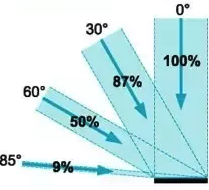
\includegraphics[width=\linewidth]{Materials/Irradiance}
		\caption{Illustration taken from \cite{quora}.}
	\end{subfigure}%
	~
	\begin{subfigure}[t]{0.45\linewidth}
		\centering
		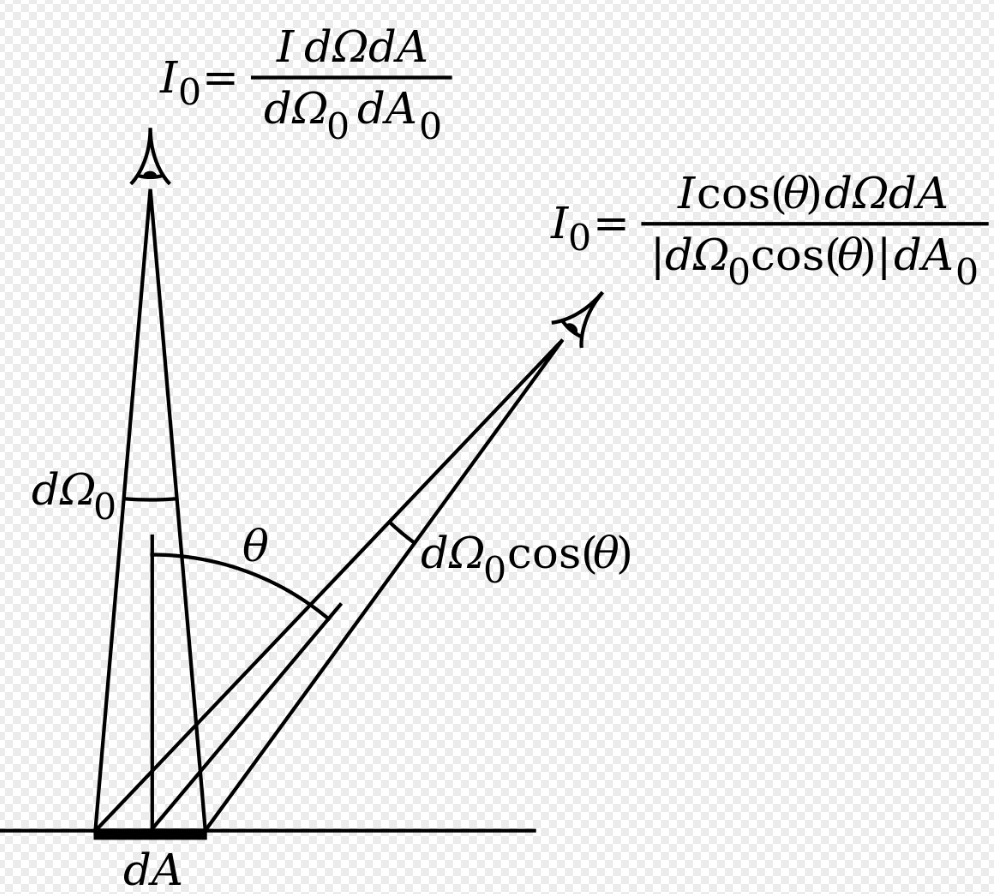
\includegraphics[width=\linewidth]{Materials/Radiance}
		\caption{Illustration taken from \cite{lamberts_law_wiki}.}
	\end{subfigure}
	\caption{As seen in (a) does the irradiance on the surface depend greatly on the angle between the illuminating source and the surface norm, but the radiance observed at different angles remains invariant as illustrated in (b).}
\end{figure}
Looking back on equation \ref{Laberts_law}, $I(p)$ denotes the intensity at the pixel \textit{p}, $\rho(x)$ the albedo at location \textit{x}, $s(x)$ the irradiance \todo{Correct?} at location \textit{x} and $n(x)$ the surface norm direction at location \textit{x}.

\subsection{How is Lambert’s law modified to deal with self shadows}
A self shadow is a shadow cast on part of a object because that part is facing the opposite direction of the light source. Given the self shadowed part of the object is facing the opposite direction of the light, the surface norm will also point in the opposite direction. This means that if $s \cdot n \leq 0$ it is a self shadow. We can thus modify Lambert's cosine law to deal with self shadows by saying:
\begin{equation*}
	I(p) = \rho(x)max(s(x) \cdot n(x), 0)
\end{equation*}

\subsection{What about cast shadows? Comment on the difference between the two}
Cast shadows are created by one object, but might 'hit' another object in the scene. Because Lambert's cosine law is describes what happens in a single pixel (i.e. is local) we can not handle cast shadows as they may not be a product of the object they 'hit'. On the contrary, given self shadows are produced by the same object which casts them, they are local issues.

\subsection{Comment on the modelling limits of Lambert’s law}
As discussed above, cast shadows can not be modelled by Lambert's cosine law. It is also assumed that the surface is somewhat diffuse, and that the light source is parallel \todo{Actual requirement, or assumption in course?}.

\subsection{How can we obtain an estimate of albedo and normals in Woodham’s approach to Photometric Stereo. Write the equation}
From \cite{woodham} we get the equation:
\begin{equation*}
	I = qNn
\end{equation*}
Where I denotes the image, \textit{q} the reflectance factor (albedo), \textit{N} the direction of incident illumination and \textit{n} the unit surface normal. The reflectance factor is then given by:
\begin{equation*}
	q = |N^{-1}I|
\end{equation*}
And the normals can be obtained by:
\begin{equation*}
	n = \left(\frac{1}{q}\right)N^{-1}I
\end{equation*}

\subsection{What should be done if one uses RANSAC. Please describe}
RANSAC is a non-deterministic algorithm used to estimate model parameters where the data contains outliers which should not contribute to the solution. The algorithm is non-deterministic in the sense that it is only guaranteed to find a reasonable solution with a certain probability. This probability increases as the number of iterations allowed in the algorithm increases. The algorithm works by randomly sample \textit{n} data points needed to estimate model parameters, and then evaluates this model by, for instance, count how many data points are within a thresholded distance to the estimated model \cite{ransac_wiki}.
\begin{figure}[H]
	\centering
	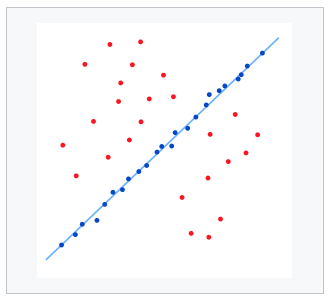
\includegraphics[width=0.5\linewidth]{Materials/Ransac}
	\caption{A fitted line with RANSAC goes through the inlier data, while the outlier data is ignored. Had a least square method been used, the line would have been skewed. Illustration from \cite{ransac_wiki}.}
\end{figure}
If one wishes to use RANSAC to estimate the normal field and albedo from a series of images, a matrix of light sources should be constructed together with a vector of pixel intensities from each image in the series, such that if there are \textit{z} images with \textit{k} pixels, one would end up with \textit{z} vectors of dimension \textit{k}. We can now use the supplied function \textit{ransac\_3dvector} which implements the RANSAC algorithm. The returned matrix can then be used to solve for the albedo and normal surface vector in that pixel, thus the RANSAC algorithm will have to be used on every pixel in the image.
\begin{thebibliography}{9}
\bibitem{book}
Forsyth, David A., Ponce, Jean. 2012. 'Computer Vision a Modern Approach'. Pearson 2nd. ed.

\bibitem{slides}
Absalon.ku.dk. 'PS.pdf'. \url{https://absalon.ku.dk/courses/36154/files/folder/Slides?preview=3307133}. Visited: December 7th 2019.

\bibitem{lamberts_law_wiki}
en.wikipedia.org. 'Lambert's cosine law'. \url{https://en.wikipedia.org/wiki/Lambert\%27s_cosine_law}. Visited: December 7th 2019.

\bibitem{ransac_wiki}
en.wikipedia.org. 'Random sample consensus'. \url{https://en.wikipedia.org/wiki/Random_sample_consensus}. Visited: December 7th 2019.

\bibitem{quora}
quora.com. 'What is Lamberts Cosine Law?'. \url{https://www.quora.com/What-is-Lamberts-Cosine-Law}. Visited: December 7th 2019.

\bibitem{woodham}
Robert J. Woodham. 1980. 'Photometric method for determining surface orientation from multiple images'. Department of Computer Science University of British Columbia.

\end{thebibliography}

\end{document}